%!TEX root = ../main.tex

\todo Write up something about the experimental setup

\section{Calibration of a multichannel analyser}
\label{sec:ecal}

\begin{figure}
	\label{fig:ecal-plot}
	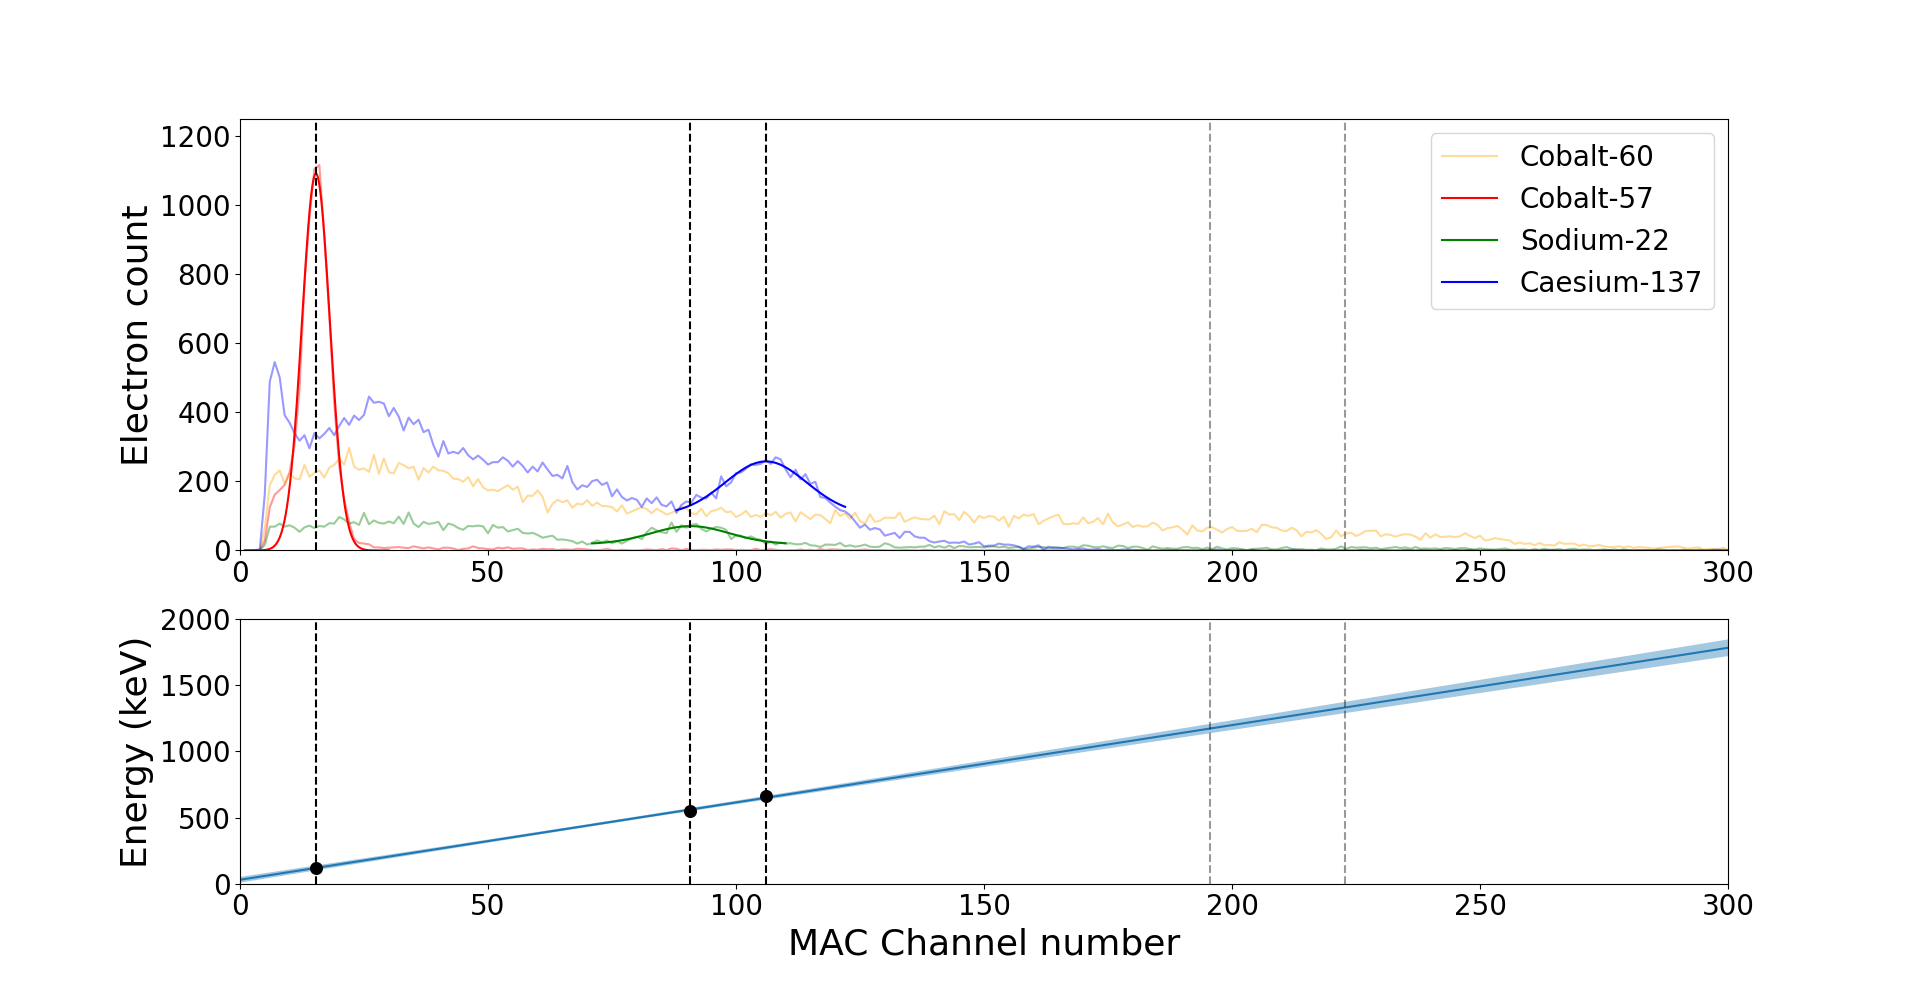
\includegraphics[width=1.0\textwidth]{./fig/ecal-plot.png}
	\caption{}{The gamma spectra of various radionuclides as measured by the MAC
	is depicted in the upper plot. A Gaussian fit hightlights the characteristic
	photopeaks for each (except Co-60, see text) measurement. The lower plot
	sets the measured channel numbers into context with the energies of the
	observed transitions. A linear model that connects MAC channel number with an
	energy is established.}
\end{figure}

As a first task the MAC needs to be calibrated so that measured channel numbers of an
event can be related to the energy of the particles that caused it. The presented
calibration is fourfold. In seperate measurements the radionuclides Cobalt-57, and
-60, as well as Sodium-22, and Caesium-137 are placed in front of the
NaJ-scintillator. Their $\gamma$-spectrum is measured for \SI{300}{\second}. The
resulting distribution of observed events across the different measuring channels is
depicted in \autoref{fig:ecal-plot}. The interesting parts of the spectra are the
gaussian shaped sections located at the tail ends. They represent the photopeaks
discussed briefly in \autoref{sec:compton-spectrum}.

Equipped with theoretical knowledge of the radioactive processes, one can compare the
measured channel with the expected energy of a nuclear transition (see \todo
\autoref{app:transitions}) to establish a linear connection between the two. For a
more solid result this calibration is done simultanously for all measured
radionuclides. A linear regression over all reference points then allows a 
quantitative analysis of measurement results. Below listed in 
\autoref{tab:transitions} are the different observed radioactive transitions, their 
characteristic transition energies, as well as the channel they were observed in by 
the MAC, the last column holds information about the location of a guassian fit 
applied to the signal. In the bottom plot of \autoref{fig:ecal-plot} these results 
are furthermore visualised.

\begin{table}
	\begin{center}
	\caption{MAC energy calibration parameters}
	\begin{tabular*}{0.9\textwidth}{@{\extracolsep{\fill}} c|crr}
		\toprule
	        \textbf{Transition} & \textbf{Energy (keV)} & \textbf{measured channel} & \textbf{fit channel} \\
		\midrule
		$^{57}$Co $\rightarrow$ $^{57}$Fe & 122.061 & 16 & 15.3(1) \\
		$^{22}$Na $\rightarrow$ $^{22}$Ne & 546.544 & 91 & 90.8(4) \\
		$^{137}$Cs $\rightarrow$ $^{137m}$Ba & 661.659 & 108 & 106.0(3) \\
		$^{60}$Co $\rightarrow$ $^{60}$Ni* & 1173.200 & - & see text \\
		$^{60}$Ni* $\rightarrow$ $^{60}$Ni & 1332.000 & - & see text \\
		\bottomrule
		\end{tabular*}
		\label{tab:ecal-params}
	\end{center}
\end{table}


As can be seen both in the plot as well as the table, a calibration for the
photopeaks of $^{60}$Co are not conducted. From the location of other photopeaks the
characteristic points of the $^{60}$Co $\gamma$spectrum should be located around
channels $\#195$ and $\#223$. This can however not be experimentally verified. A
reasonable analysis cannot be completed, as the photopeaks are - provided the
presented methodology is sound - far too faint. This can perhaps be prevented in 
future lab assignments by gathering more data of the $^{60}$Co spectrum.

In any case, a linear model that connects channel number $\mathcal{C}$ to a particle
energy $E$ is obtained. They can be related to each other via \autoref{eq:ecal-eq}
that is presented below.

\begin{equation}
\label{eq:ecal-eq}
	E(\mathcal{C}) = \underbrace{\SI{5.8\pm0.3}{\kilo\electronvolt}}_\text{a}\cdot\;\mathcal{C} + \underbrace{\SI{30.2\pm22.0}{\kilo\electronvolt}}_\text{b}
\end{equation}

Albeit only three of the four radionuclides can be used effectively for a
calibration, the results nevertheless seem promising. A quick check regarding the
goodness of fit finds a reduced $\chi^{2}_\nu\approx0.97$, indicating that the model
conforms with observations to reasonable accuracy. This accuracy $\Delta E
(\mathcal{C})$ can then be quantified using the covariance matrix $\text{COV}(a,b)$, 
estimated by the fitting algorithm, as well as the gradient $\nabla E$, which can
easily be calculated by hand.

\begin{equation}
	\text{COV}(a,b) =
	\left[
	\begin{array}{c c}
	0.0736 & -5.2014 \\
	-5.2014 & 483.5527
	\end{array}
	\right],
	\qquad\nabla E = \begin{pmatrix}\mathcal{C}\\1\end{pmatrix}.
\end{equation}

With the above quantities, the error in the estimated energy then propagates like:

\begin{equation}
\label{eq:energy-error}
	\Delta E(\mathcal{C}) = \sqrt{\,(\nabla E)^{T}\,\text{COV}(a,b)\,\nabla E}\,.
\end{equation}
